\documentclass[10pt,a4paper]{article}
\usepackage{amsmath}
\usepackage[
    colorlinks,
    citecolor=blue!70!black,
    linkcolor=blue!70!black,
    urlcolor=blue!70!black
]{hyperref}
\usepackage{tikz}
\usetikzlibrary{patterns}
\usepackage{xcolor}

\newcommand{\hexgrid}[3]{
    \draw[dotted,gray] (#1-#3,#2+#3) -- (#1+#3,#2+#3);

    \draw[dotted,gray] (#1,#2) -- (#1,#2+2*#3);

    \draw[dotted,gray] (#1+#3,#2) -- (#1-#3,#2+2*#3);

    \foreach \i in {1,...,#3} {
        \draw[dotted,gray] (#1-#3,#2+#3+\i) -- (#1+#3-\i,#2+#3+\i);
        \draw[dotted,gray] (#1-#3+\i,#2+#3-\i) -- (#1+#3,#2+#3-\i);

        \draw[dotted,gray] (#1+\i,#2) -- (#1+\i,#2+2*#3-\i);
        \draw[dotted,gray] (#1-\i,#2+\i) -- (#1-\i,#2+2*#3);

        \draw[dotted,gray] (#1+#3-\i,#2) -- (#1-#3,#2+2*#3-\i);
        \draw[dotted,gray] (#1+#3,#2+\i) -- (#1-#3+\i,#2+2*#3);
    }
}

\begin{document}

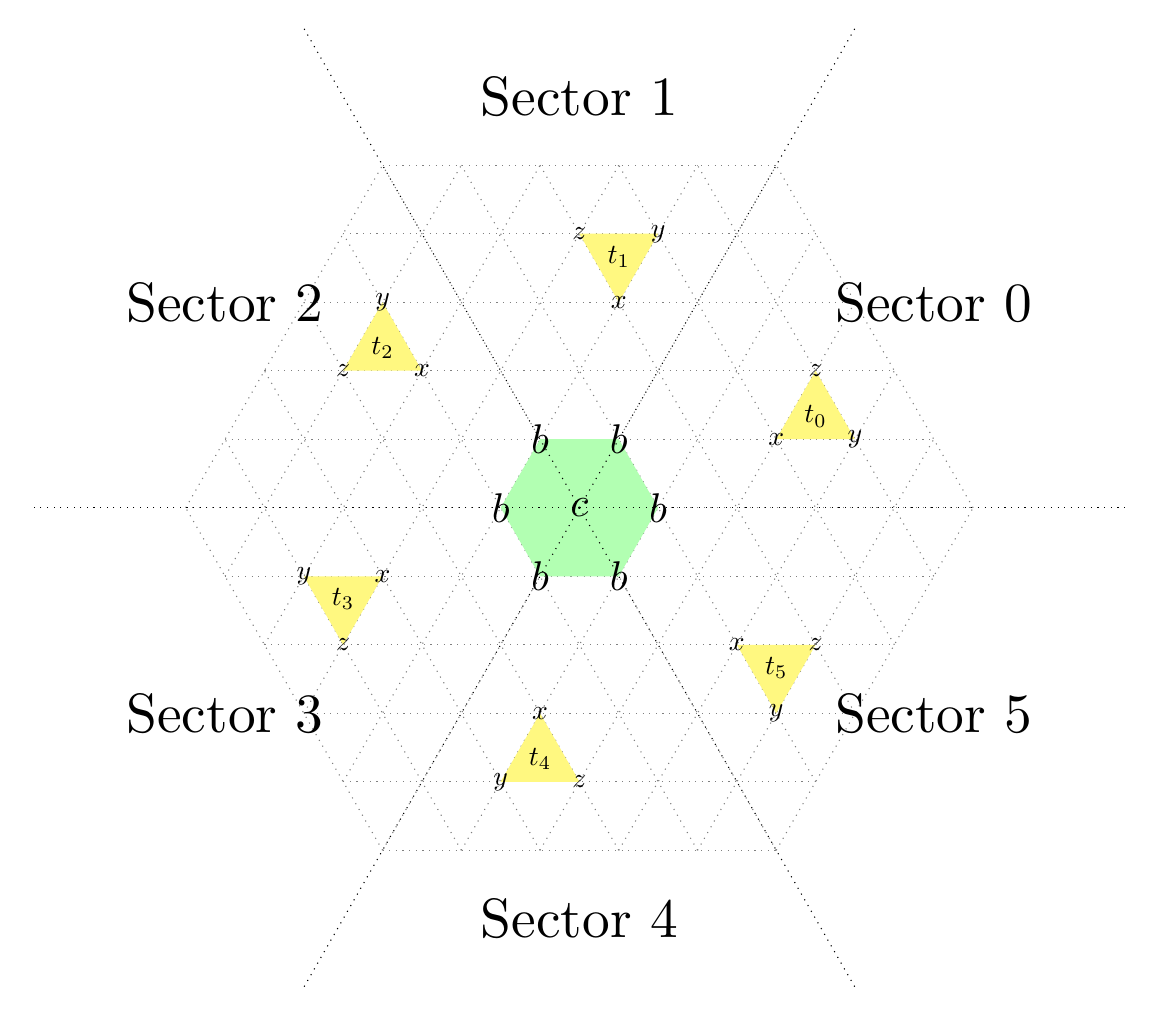
\begin{tikzpicture}
    	\begin{scope}[yscale=.87,xslant=.5]
        \hexgrid{0}{-5}{5};

        \fill[green!30] (1,0) -- (0,1) -- (-1,1) -- (-1,0) -- (0,-1) -- (1,-1) -- cycle;

                \draw[dotted] (0,0) -- (7,0);
        \node[scale=2] at (3,3) {Sector $0$};
        \fill[yellow!50] (2,1) -- (3,1) -- (2,2) -- cycle;
        \node at (7/3,4/3) {$t_0$};
        \node at (2,1) {$x$};
        \node at (3,1) {$y$};
        \node at (2,2) {$z$};
        \draw[dotted] (0,0) -- (0,7);
        \node[scale=2] at (-3,6) {Sector $1$};
        \fill[yellow!50] (-1,3) -- (-1,4) -- (-2,4) -- cycle;
        \node at (-4/3,11/3) {$t_1$};
        \node at (-1,3) {$x$};
        \node at (-1,4) {$y$};
        \node at (-2,4) {$z$};
        \draw[dotted] (0,0) -- (-7,7);
        \node[scale=2] at (-6,3) {Sector $2$};
        \fill[yellow!50] (-3,2) -- (-4,3) -- (-4,2) -- cycle;
        \node at (-11/3,7/3) {$t_2$};
        \node at (-3,2) {$x$};
        \node at (-4,3) {$y$};
        \node at (-4,2) {$z$};
        \draw[dotted] (0,0) -- (-7,0);
        \node[scale=2] at (-3,-3) {Sector $3$};
        \fill[yellow!50] (-2,-1) -- (-3,-1) -- (-2,-2) -- cycle;
        \node at (-7/3,-4/3) {$t_3$};
        \node at (-2,-1) {$x$};
        \node at (-3,-1) {$y$};
        \node at (-2,-2) {$z$};
        \draw[dotted] (0,0) -- (0,-7);
        \node[scale=2] at (3,-6) {Sector $4$};
        \fill[yellow!50] (1,-3) -- (1,-4) -- (2,-4) -- cycle;
        \node at (4/3,-11/3) {$t_4$};
        \node at (1,-3) {$x$};
        \node at (1,-4) {$y$};
        \node at (2,-4) {$z$};
        \draw[dotted] (0,0) -- (7,-7);
        \node[scale=2] at (6,-3) {Sector $5$};
        \fill[yellow!50] (3,-2) -- (4,-3) -- (4,-2) -- cycle;
        \node at (11/3,-7/3) {$t_5$};
        \node at (3,-2) {$x$};
        \node at (4,-3) {$y$};
        \node at (4,-2) {$z$};
 
        \node[scale=1.5] at (0,0) {$c$};
        \node[scale=1.5] at (1,0) {$b$};
        \node[scale=1.5] at (0,1) {$b$};
        \node[scale=1.5] at (-1,1) {$b$};
        \node[scale=1.5] at (-1,0) {$b$};
        \node[scale=1.5] at (0,-1) {$b$};
        \node[scale=1.5] at (1,-1) {$b$};
    	\end{scope}
    \end{tikzpicture}

\end{document}